\subsection{Compactness and Completeness}\label{subsec:compactness-and-completeness}

% **Role:** abstract structure behind limits and continuity.
%
% Compactness, sequential compactness in metric spaces, Heine--Borel, completeness, total boundedness, Baire category.


Compactness extracts finite or convergent structure from infinite behavior; completeness asks whether Cauchy approximations converge internally.

\begin{definition} \label{def:open-cover-and-compactness} \hlt{Open Covers and Compact Sets}\\
Let $E\subseteq X$, where $X$ is a metric space.\\
An \hlt{open cover} of $E$ is a collection $\{G_\alpha\}_{\alpha\in A}$ of open subsets of $X$ such that $E\subseteq\bigcup\limits_{\alpha\in A}G_\alpha$. A set $K\subseteq X$ is \hlt{compact} if every open cover of $K$ has a finite subcover: $K\subseteq G_{\alpha_1}\cup\cdots\cup G_{\alpha_n}$ for some finite subcollection.
\end{definition}

\begin{figure}[H]
  \centering
  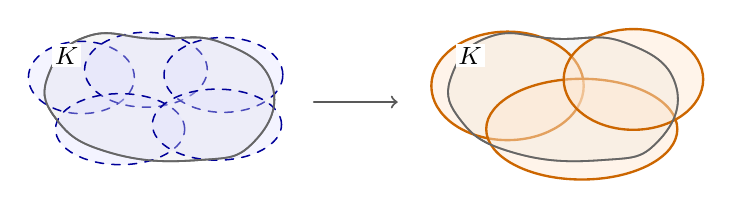
\begin{tikzpicture}[
  scale=0.82,
  every node/.style={font=\small},
  line cap=round,
  line join=round,
  compact/.style={draw=black!60, fill=gray!8, line width=0.65pt},
  compactoutline/.style={draw=black!60, line width=0.65pt},
  cover/.style={draw=blue!60!black, fill=blue!12, fill opacity=0.34, dashed, line width=0.55pt},
  chosen/.style={draw=orange!80!black, fill=orange!18, fill opacity=0.46, line width=0.85pt},
  arrow/.style={->, black!65, line width=0.75pt},
  note/.style={fill=white, inner sep=1pt}
]
  \begin{scope}
    \draw[compact]
      plot[smooth cycle, tension=0.8] coordinates {
        (-1.75,0.45) (-1.15,1.02) (-0.15,0.98) (0.92,0.92)
        (1.70,0.28) (1.42,-0.62) (0.55,-0.9) (-0.82,-0.78)
        (-1.65,-0.25)
      };
    \foreach \x/\y/\rx/\ry in {-1.25/0.38/0.82/0.56,-0.25/0.5/0.95/0.58,0.95/0.42/0.92/0.58,-0.65/-0.42/1.0/0.55,0.85/-0.35/1.0/0.55} {
      \draw[cover] (\x,\y) ellipse ({\rx} and {\ry});
    }
    \draw[compactoutline]
      plot[smooth cycle, tension=0.8] coordinates {
        (-1.75,0.45) (-1.15,1.02) (-0.15,0.98) (0.92,0.92)
        (1.70,0.28) (1.42,-0.62) (0.55,-0.9) (-0.82,-0.78)
        (-1.65,-0.25)
      };
    \node[note] at (-1.48,0.72) {$K$};
  \end{scope}

  \draw[arrow] (2.35,0) -- (3.65,0);

  \begin{scope}[xshift=6.25cm]
    \draw[compact]
      plot[smooth cycle, tension=0.8] coordinates {
        (-1.75,0.45) (-1.15,1.02) (-0.15,0.98) (0.92,0.92)
        (1.70,0.28) (1.42,-0.62) (0.55,-0.9) (-0.82,-0.78)
        (-1.65,-0.25)
      };
    \draw[chosen] (-0.9,0.25) ellipse (1.18 and 0.84);
    \draw[chosen] (0.25,-0.42) ellipse (1.48 and 0.78);
    \draw[chosen] (1.05,0.35) ellipse (1.08 and 0.78);
    \draw[compactoutline]
      plot[smooth cycle, tension=0.8] coordinates {
        (-1.75,0.45) (-1.15,1.02) (-0.15,0.98) (0.92,0.92)
        (1.70,0.28) (1.42,-0.62) (0.55,-0.9) (-0.82,-0.78)
        (-1.65,-0.25)
      };
    \node[note] at (-1.48,0.72) {$K$};
  \end{scope}
\end{tikzpicture}

  \caption{Compactness extracts a finite subcover.}
  \label{fig:compactness-finite-subcover}
\end{figure}

\begin{definition} \label{def:sequentially-compact-metric-space} \hlt{Sequential Compactness}\\
A metric space is \hlt{sequentially compact} if every sequence has a convergent subsequence.
\end{definition}

\begin{theorem} \label{thm:compact-sequential-subsequence} \hlt{Compactness Produces Convergent Subsequences}
\begin{enumerate}[label=(\roman*)]
\setlength{\itemsep}{0pt}
\item If $(p_n)$ is a sequence in a compact metric space $X$, then $p_{n_i}\to p$ for some subsequence and some $p\in X$.
\item If $(\mathbf{x}_n)$ is bounded in $\R^k$, then it has a convergent subsequence.
\end{enumerate}
\begin{proof}
\begin{enumerate}[label=(\roman*)]
\setlength{\itemsep}{0pt}
\item Let $E=\{p_n:n\in\N\}$. If $E$ is finite, choose a value $p$ attained infinitely often; the corresponding constant subsequence converges. If $E$ is infinite, Theorem \ref{thm:infinite-subset-of-compact-has-limit-point} gives a limit point $p\in X$ of $E$. By Theorem \ref{thm:limit-point-neighborhoods-infinitely-many}, choose $n_i>n_{i-1}$ with $d(p_{n_i},p)<1/i$. Then $p_{n_i}\to p$.
\item The range of $(\mathbf{x}_n)$ has compact closure by Theorem \ref{thm:heine-borel-rk}; apply (i) in that closure.
\end{enumerate}
\hlt{Structural Commentary}: Compactness turns arbitrary infinite behavior into an accumulating subsequence.\\
\hlt{Key Insight}: In $\R^k$, boundedness is enough because bounded sets sit inside compact closed cells.
\end{proof}
\end{theorem}

\begin{theorem} \label{thm:subsequential-limits-closed} \hlt{Subsequential Limits Form a Closed Set}\\
For a sequence $(p_n)$ in a metric space $X$, the set of all subsequential limits is closed.
\begin{proof}
Let $E^*$ be the set of subsequential limits and let $q$ be a limit point of $E^*$. Set $n_0=0$.\\
For each $i$, choose $x_i\in E^*$ with $d(x_i,q)<2^{-i}$. Since $x_i$ is a subsequential limit, choose $n_i>n_{i-1}$ such that $d(p_{n_i},x_i)<2^{-i}$. Then $d(p_{n_i},q)<2^{1-i}$, so $p_{n_i}\to q$, and $q\in E^*$.\\
\hlt{Structural Commentary}: A limit of subsequential limits is reached by diagonalizing through those subsequences.\\
\hlt{Key Insight}: Choose later and closer terms at the same time.
\end{proof}
\end{theorem}

\begin{definition} \label{def:cauchy-sequence} \hlt{Cauchy Sequence}\\
A sequence $(p_n)$ in a metric space $X$ is \hlt{Cauchy} if $\forall \varepsilon>0$  $\exists$ integer $N$ s.t. $n\geq N,\ m\geq N$ $\Longrightarrow$ $d(p_n,p_m)<\varepsilon$.
\end{definition}

\begin{definition} \label{def:diameter-of-metric-set} \hlt{Diameter}\\
Let $E$ be a nonempty subset of a metric space $X$. The \hlt{diameter} of $E$ is $\diam E\defeq\sup\{d(p,q):p,q\in E\}$, with the supremum interpreted in the extended real sense when the set of distances is unbounded.
\end{definition}

\begin{proposition} \label{prop:diameter-basic-properties} \hlt{Basic Diameter Properties}\\
Let $\emptyset\ne E,F\subseteq X$.
\begin{enumerate}[label=(\roman*)]
\setlength{\itemsep}{0pt}
\item $E$ is bounded $\Longleftrightarrow\diam E<\infty\Longleftrightarrow\exists q\in X,\exists M>0$ such that $E\subseteq B_M(q)$.
\item $\diam E=0\Longleftrightarrow |E|=1$.
\item $E\subseteq F\Longrightarrow\diam E\leq\diam F$.
\item $E,F$ bounded $\Longrightarrow E\cup F$ bounded.
\end{enumerate}
\begin{proof}
\begin{enumerate}[label=(\roman*)]
\setlength{\itemsep}{0pt}
\item If $E\subseteq B_M(q)$, then $d(x,y)\leq d(x,q)+d(q,y)<2M$ for $x,y\in E$, so $\diam E<\infty$.\\
If $\diam E<\infty$ and $q\in E$, then $E\subseteq B_{\diam E+1}(q)$.
\item $\diam E=0\Longleftrightarrow d(x,y)=0$ for all $x,y\in E\Longleftrightarrow x=y$ for all $x,y\in E$; since $E\ne\emptyset$, this is $|E|=1$.
\item $\{d(x,y):x,y\in E\}\subseteq\{d(x,y):x,y\in F\}$, so monotonicity of $\sup$ gives $\diam E\leq\diam F$.
\item Choose $e\in E$, $f\in F$, and set $D\defeq\diam E+d(e,f)+\diam F<\infty$. For $x,y\in E\cup F$, either $x,y$ lie in the same set, or after swapping, $x\in E$, $y\in F$, and $d(x,y)\leq d(x,e)+d(e,f)+d(f,y)\leq D$.\\
Thus $\diam(E\cup F)<\infty$, so $E\cup F$ is bounded by (i).
\end{enumerate}
\hlt{Structural Commentary}: Diameter is a single-number form of boundedness for nonempty sets.\\
\hlt{Key Insight}: Cross-distances between two bounded sets are controlled by one bridge distance.
\end{proof}
\end{proposition}

\begin{proposition} \label{prop:cauchy-tail-diameters} \hlt{Cauchy Sequences and Tail Diameters}\\
For $(p_n)$ in a metric space $X$, set $E_N\defeq\{p_j:j\geq N\}$. Then $(p_n)$ is Cauchy if and only if $\diam E_N\to0$.
\begin{proof}
\begin{enumerate}[label=\roman*.]
\setlength{\itemsep}{0pt}
\item[$(\Rightarrow)$] Given $\varepsilon>0$, choose $N_0$ so that $m,n\geq N_0$ implies $d(p_m,p_n)<\varepsilon/2$.\\
If $N\geq N_0$, then every pair in $E_N$ has distance $<\varepsilon/2$, so $\diam E_N<\varepsilon$.
\item[$(\Leftarrow)$] Given $\varepsilon>0$, choose $N_0$ with $\diam E_{N_0}<\varepsilon$.\\
If $m,n\geq N_0$, then $p_m,p_n\in E_{N_0}$, hence $d(p_m,p_n)\leq\diam E_{N_0}<\varepsilon$.
\end{enumerate}
\hlt{Structural Commentary}: Cauchy behavior is shrinking diameter of sequence tails.\\
\hlt{Key Insight}: The limit is not named; only mutual closeness is measured.
\end{proof}
\end{proposition}

\begin{figure}[H]
  \centering
  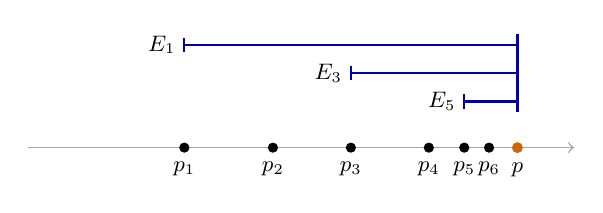
\begin{tikzpicture}[
  scale=0.90,
  transform shape,
  every node/.style={font=\small},
  axis/.style={->, gray!70, line width=0.55pt},
  tail/.style={blue!70!black, line width=0.8pt},
  dot/.style={circle, fill=black, inner sep=1.45pt},
  limit/.style={circle, fill=orange!80!black, inner sep=1.55pt}
]
  \draw[axis] (-0.2,0) -- (7.5,0);
  \node[limit,label=below:$p$] at (6.7,0) {};

  \foreach \x/\lab in {2.0/p_1,3.25/p_2,4.35/p_3,5.45/p_4,5.95/p_5,6.30/p_6} {
    \node[dot,label=below:\(\lab\)] at (\x,0) {};
  }

  \draw[tail] (2.0,1.45) -- (6.7,1.45);
  \draw[tail] (4.35,1.05) -- (6.7,1.05);
  \draw[tail] (5.95,0.65) -- (6.7,0.65);

  \node[left] at (2.0,1.45) {$\diam E_1$};
  \node[left] at (4.35,1.05) {$\diam E_3$};
  \node[left] at (5.95,0.65) {$\diam E_5$};

  \draw[tail] (2.0,1.35) -- (2.0,1.55);
  \draw[tail] (4.35,0.95) -- (4.35,1.15);
  \draw[tail] (5.95,0.55) -- (5.95,0.75);
  \draw[tail] (6.7,0.5) -- (6.7,1.6);
\end{tikzpicture}

  \caption{Tail diameters $\diam E_N$ shrink toward $0$.}
  \label{fig:cauchy-tail-diameters}
\end{figure}

\begin{theorem} \label{thm:nested-compact-diameters-singleton} \hlt{Nested Compact Sets with Shrinking Diameter}\\
Let $X$ be a metric space.
\begin{enumerate}[label=(\roman*)]
\setlength{\itemsep}{0pt}
\item If $\emptyset\ne E\subseteq X$, then $\diam\overline{E}=\diam E$.
\item If $K_1\supseteq K_2\supseteq\cdots$ are nonempty compact subsets of $X$ and $\diam K_n\to0$, then $\abs{\bigcap_{n=1}^{\infty}K_n}=1$.
\end{enumerate}
\begin{proof}
\begin{enumerate}[label=(\roman*)]
\setlength{\itemsep}{0pt}
\item Since $E\subseteq\overline{E}$, $\diam E\leq\diam\overline{E}$. For $p,q\in\overline{E}$ and $\varepsilon>0$, choose $p',q'\in E$ with $d(p,p'),d(q,q')<\varepsilon$; then $d(p,q)\leq\diam E+2\varepsilon$. Hence $\diam\overline{E}\leq\diam E$.
\item Set $I\defeq\bigcap_{n\geq1}K_n$. Corollary \ref{cor:nested-nonempty-compact-intersection} gives $I\ne\emptyset$. If $x,y\in I$, then $d(x,y)\leq\diam K_n$ for all $n$, so $d(x,y)=0$ as $\diam K_n\to0$. Thus $x=y$, hence $\abs I=1$.
\end{enumerate}
\hlt{Structural Commentary}: Closure preserves $\diam$; $K_n\downarrow$ with $\diam K_n\to0$ forces a singleton.\\
\hlt{Key Insight}: Compactness gives existence; shrinking diameter gives uniqueness.
\end{proof}
\end{theorem}

\begin{theorem} \label{thm:cauchy-convergence-criterion}\label{thm:sequences-completeness-main-source-todo} \hlt{Cauchy Criterion and Completeness Results}
\begin{enumerate}[label=(\roman*)]
\setlength{\itemsep}{0pt}
\item In any metric space, every convergent sequence is Cauchy.
\item If $X$ is a compact metric space, then every Cauchy sequence in $X$ converges to a point of $X$.
\item In $\R^k$, every Cauchy sequence converges.
\end{enumerate}
\begin{proof}
\begin{enumerate}[label=(\roman*)]
\setlength{\itemsep}{0pt}
\item If $p_n\to p$, choose $N$ with $d(p_n,p)<\varepsilon/2$ for $n\geq N$. For $m,n\geq N$, $d(p_n,p_m)<\varepsilon$.
\item Let $E_N\defeq\{p_j:j\geq N\}$ and $F_N\defeq\overline{E_N}$. Then $\diam F_N\to0$, the $F_N$ are compact and nested, and Theorem \ref{thm:nested-compact-diameters-singleton} gives $\bigcap_NF_N=\{p\}$. If $\diam F_N<\varepsilon$, then $p,p_n\in F_N$ for $n\geq N$, so $d(p_n,p)<\varepsilon$.
\item For Cauchy $(\mathbf{x}_n)\subseteq\R^k$, choose $N$ with $\diam\{\mathbf{x}_j:j\geq N\}<1$. Its range is bounded, hence has compact closure by Theorem \ref{thm:heine-borel-rk}; apply (ii).
\end{enumerate}
\hlt{Structural Commentary}: Cauchy controls $\diam E_N$; compactness turns $\bigcap_NF_N$ into the limit.\\
\hlt{Key Insight}: In $\R^k$, the Cauchy criterion is equivalent to convergence.
\end{proof}
\end{theorem}

\begin{lemma} \label{lem:cauchy-sequence-with-convergent-subsequence} \hlt{A Cauchy Sequence with a Convergent Subsequence Converges}\\
Let $(p_n)$ be a Cauchy sequence in a metric space $X$. If some subsequence $(p_{n_j})$ converges to $p\in X$, then $p_n\to p$.
\begin{proof}
Given $\varepsilon>0$, choose $N_0$ so that $m,n\geq N_0$ implies $d(p_m,p_n)<\varepsilon/2$.\\
Choose $j$ with $n_j\geq N_0$ and $d(p_{n_j},p)<\varepsilon/2$. Then for every $n\geq N_0$, $d(p_n,p)\leq d(p_n,p_{n_j})+d(p_{n_j},p)<\varepsilon$.\\
\hlt{Structural Commentary}: The Cauchy tail follows any convergent subsequence to the same limit.\\
\hlt{Key Insight}: Mutual closeness plus one convergent thread forces the whole tail to converge.
\end{proof}
\end{lemma}

\begin{proposition} \label{prop:cauchy-sequences-bounded-distance-converges} \hlt{Boundedness and Distances of Cauchy Sequences}\\
Let $(p_n),(q_n)$ be Cauchy sequences in a metric space $X$.
\begin{enumerate}[label=(\roman*)]
\setlength{\itemsep}{0pt}
\item \hlt{Cauchy boundedness}: the range of $n\mapsto p_n$, $\operatorname{ran}(p_n)\defeq\{p_n:n\in\N\}$ is bounded.
\item \hlt{distance convergence}: the sequence $n\mapsto d(p_n,q_n)$ converges in $\R$.
\item \hlt{nonconverse}: there exists a bounded sequence in $\R$ that is not Cauchy.
\end{enumerate}
\begin{proof}
\begin{enumerate}[label=(\roman*)]
\setlength{\itemsep}{0pt}
\item Choose $N$ with $m,n\geq N\Longrightarrow d(p_m,p_n)<1$.\\
Then $\{p_n:n\geq N\}\subseteq B_1(p_N)$, and $\{p_1,\ldots,p_{N-1}\}$ is finite, so $\operatorname{ran}(p_n)$ is bounded.
\item For $m,n\in\N$, $\abs{d(p_n,q_n)-d(p_m,q_m)}\leq d(p_n,p_m)+d(q_n,q_m)$. Hence $(d(p_n,q_n))$ Cauchy in $\R$, converges.
\item Let $a_n\defeq(-1)^n$. Then $\abs{a_n}\leq1$ for all $n$, but with $\varepsilon=1$, for every $N$ there exist $m,n\geq N$ with $\abs{a_m-a_n}=2$; hence $(a_n)$ is bounded but not Cauchy.
\end{enumerate}
\hlt{Structural Commentary}: Cauchy tails are bounded; Cauchy-pair distances converge.\\
\hlt{Key Insight}: The four-point triangle estimate controls distance sequences.
\end{proof}
\end{proposition}

\begin{definition} \label{def:complete-metric-space} \hlt{Complete Metric Space}\\
A metric space $X$ is \hlt{complete} if every Cauchy sequence in $X$ converges to a point of $X$.\\
Compact metric spaces and $\R^k$ are complete (by Theorem \ref{thm:cauchy-convergence-criterion}).
\end{definition}

\begin{proposition} \label{prop:basic-completeness-consequences} \hlt{Completeness and Closed Subspaces}\\
Let $(X,d)$ be a metric space, $E\subseteq X$, and $d_E:=d|_{E\times E}$.
\begin{enumerate}[label=(\roman*)]
\setlength{\itemsep}{0pt}
\item If $(E,d_E)$ is complete, then $E$ is closed in $X$, equivalently $E=\overline{E}^{\,X}$.
\item If $(X,d)$ is complete, then $(E,d_E)$ is complete if and only if $E$ is closed in $X$, equivalently $E=\overline{E}^{\,X}$.
\end{enumerate}
\begin{proof}
\begin{enumerate}[label=(\roman*)]
\setlength{\itemsep}{0pt}
\item Assume $(E,d_E)$ complete. Let $p\in\overline{E}^{\,X}$. Choose $(p_n)\subseteq E$ with $d(p_n,p)<1/n$.\\
Then $p_n\to p$ in $X$, hence $(p_n)$ is Cauchy in $(E,d_E)$. Thus $p_n\to q\in E$ in $(E,d_E)$, hence also in $X$.\\
Uniqueness in $X$ gives $p=q\in E$. Therefore $\overline{E}^{\,X}\subseteq E$, so $E=\overline{E}^{\,X}$.
\item Assume $(X,d)$ complete. By (i), $(E,d_E)$ complete $\Rightarrow E=\overline{E}^{\,X}$.\\
Conversely, if $E=\overline{E}^{\,X}$ and $(p_n)\subseteq E$ is Cauchy in $(E,d_E)$, then $(p_n)$ is Cauchy in $X$, so $p_n\to p\in X$.\\
Since $p\in\overline{E}^{\,X}=E$, every Cauchy sequence in $(E,d_E)$ converges in $(E,d_E)$.
\end{enumerate}
\hlt{Structural Commentary}: Completeness gives the limit in $X$; closedness keeps it in $E$.\\
\hlt{Key Insight}: In a complete ambient space, $E$ is complete exactly when $\overline{E}=E$.
\end{proof}
\end{proposition}

\begin{example} \label{ex:finite-dimensional-complete-metric-spaces} \hlt{Finite-Dimensional Complete Metric Spaces}\\
For $k\in\N$, $(\R^k,d_2)$ and $(\C^k,d_2)$ are complete; in particular, so are $\R$ and $\C$.
\begin{proof}
Completeness of $\R$ is Theorem \ref{thm:real-cauchy-convergence-criterion}.\\
If $z_n=x_n+iy_n$ is Cauchy in $\C$, then $(x_n)$ and $(y_n)$ are Cauchy in $\R$, so $z_n\to x+iy\in\C$.\\
Theorem \ref{thm:cauchy-convergence-criterion} gives completeness of $\R^k$, and the isometry $\C^k\cong\R^{2k}$ gives completeness of $\C^k$.\\
\hlt{Structural Commentary}: Finite-dimensional completeness is coordinatewise completeness.\\
\hlt{Key Insight}: A Cauchy sequence in finitely many coordinates converges coordinate by coordinate.
\end{proof}
\end{example}

\begin{example} \label{ex:continuous-functions-sup-complete-integral-not-complete} \hlt{Two Metrics on $C[0,1]$}\\
For $\mathbb{F}\in\{\R,\C\}$, $C_{\mathbb{F}}:=C([0,1],\mathbb{F})$ is complete under $d_\infty(f,g):=\sup_{x\in[0,1]}\abs{f(x)-g(x)}$ by Theorem \ref{thm:complete-supremum-metric-space}, but not under $d_1(f,g):=\int_0^1\abs{f(x)-g(x)}\,dx$.
\begin{proof}
For $n\ge2$, define $f_n\in C_{\mathbb{F}}$ by
\begin{equation*}
f_n(x)\defeq
\begin{cases}
0,&0\le x\le \frac12,\\
n(x-\frac12),&\frac12\le x\le \frac12+\frac1n,\\
1,&\frac12+\frac1n\le x\le1.
\end{cases}
\end{equation*}
Let $s:=\mathbf{1}_{(1/2,1]}$. Then $d_1(f_n,s)=1/(2n)$, hence $(f_n)$ is $d_1$-Cauchy. If $f_n\to g\in C_{\mathbb{F}}$ in $d_1$, then $d_1(g,s)=0$, so $g=s$ a.e. Continuity forces $g=0$ on $[0,1/2]$ and $g=1$ on $(1/2,1]$, impossible at $1/2$.\\
\hlt{Structural Commentary}: The integral metric permits a continuous ramp to collapse to a jump.\\
\hlt{Key Insight}: Supremum control preserves continuity; integral control can miss jumps.
\end{proof}
\end{example}

\begin{figure}[H]
  \centering
  % Source guide: Roman, Advanced Linear Algebra, Ch. 12, Figure 12.3.
% Redrawn to show the continuous ramps that converge in the integral metric
% to a discontinuous step function.
\begin{tikzpicture}[
  x=5.4cm,
  y=2.05cm,
  >=Stealth,
  every node/.style={font=\scriptsize},
  axis/.style={->, gray!75, line width=0.55pt},
  graph/.style={blue!70!black, line width=0.95pt},
  limit/.style={orange!80!black, line width=0.8pt, dashed},
  tick/.style={gray!75, line width=0.45pt},
  guide/.style={gray!45, dashed, line width=0.4pt},
  labelbox/.style={fill=white, inner sep=1.2pt}
]
  \draw[axis] (-0.05,0) -- (1.08,0) node[right] {$x$};
  \draw[axis] (0,-0.08) -- (0,1.22) node[above] {$y$};

  \draw[tick] (0.5,0.035) -- (0.5,-0.035) node[below=2pt] {$\frac12$};
  \draw[tick] (1,0.035) -- (1,-0.035) node[below=2pt] {$1$};
  \draw[tick] (0.035,1) -- (-0.035,1) node[left=2pt] {$1$};
  \draw[guide] (0.68,0) -- (0.68,1);

  \draw[limit] (0,0) -- (0.5,0);
  \draw[limit] (0.5,1) -- (1,1);
  \draw[limit] (0.5,0) -- (0.5,1);
  \node[text=orange!80!black, labelbox, anchor=west] at (0.74,0.82) {step limit};

  \draw[graph] (0,0) -- (0.5,0) -- (0.68,1) -- (1,1);
  \node[text=blue!70!black, labelbox] at (0.57,0.70) {$f_n$};

  \draw[<->, teal!70!black, line width=0.55pt] (0.5,1.12) -- (0.68,1.12)
    node[midway, above=1pt, labelbox] {$1/n$};
\end{tikzpicture}

  \caption{The continuous ramps $f_n$ converge in the integral metric to a
  discontinuous step function.}
  \label{fig:continuous-functions-integral-metric-not-complete}
\end{figure}

\begin{example} \label{ex:sequence-spaces-complete} \hlt{Completeness of $\ell^\infty$ and $\ell^p$}\\
For $\mathbb{F}\in\{\R,\C\}$, $(\ell^\infty(\mathbb{F}),\norm{\cdot}_\infty)$ and $(\ell^p(\mathbb{F}),\norm{\cdot}_p)$, $1\leq p<\infty$, are complete.
\begin{proof}
For $\ell^\infty$, let $\mathbf{x}^{(n)}=(x_j^{(n)})_j$ be Cauchy. Then $x_j^{(n)}\to y_j\in\mathbb{F}$ for each $j$.\\
If $\norm{\mathbf{x}^{(n)}-\mathbf{x}^{(m)}}_\infty<\varepsilon$ for $m,n\geq N$, then $\abs{x_j^{(n)}-y_j}\leq\varepsilon$ for all $j$, so $\norm{\mathbf{x}^{(n)}-\mathbf{y}}_\infty\leq\varepsilon$.\\
Taking $n=N$ gives $\mathbf{y}\in\ell^\infty$, hence $\mathbf{x}^{(n)}\to\mathbf{y}$.\\
For $\ell^p$, let $\mathbf{x}^{(n)}$ be Cauchy and define $\mathbf{y}=(y_j)$ by coordinatewise limits.\\
If $\norm{\mathbf{x}^{(n)}-\mathbf{x}^{(m)}}_p<\varepsilon$ for $m,n\geq N$, then for each $r$, $\sum\limits_{j=1}^{r}\abs{x_j^{(n)}-y_j}^{p}=\lim\limits_{m\to\infty}\sum\limits_{j=1}^{r}\abs{x_j^{(n)}-x_j^{(m)}}^{p}\leq\varepsilon^p$.\\
Letting $r\to\infty$ gives $\norm{\mathbf{x}^{(n)}-\mathbf{y}}_p\leq\varepsilon$ for $n\geq N$. Taking $n=N$ gives $\mathbf{y}\in\ell^p$, hence $\mathbf{x}^{(n)}\to\mathbf{y}$.\\
\hlt{Structural Commentary}: Completeness of scalar coordinates combines with uniform tail control.\\
\hlt{Key Insight}: Norm-Cauchy control keeps coordinatewise limits inside the space.
\end{proof}
\end{example}

\begin{definition} \label{def:contraction-mapping} \hlt{Contraction}\\
Let $X$ be a metric space with metric $d$.\\
A map $\varphi:X\to X$ is a \hlt{contraction} if $\exists$ a constant $0\leq c<1$ such that $d(\varphi(x),\varphi(y))\leq c\,d(x,y)$ for $x,y\in X$.\\
\hlt{Structural Commentary}: Bound $c<1$ excludes nonexpansive maps and is the hypothesis in Theorem \ref{thm:contraction-principle}.
\end{definition}

\begin{figure}[H]
  \centering
  \begin{tikzpicture}[
  scale=0.90,
  >=Stealth,
  every node/.style={font=\small},
  frame/.style={draw=black!60, line width=0.6pt},
  image/.style={fill=gray!17, draw=black!60, line width=0.7pt},
  inward/.style={->, black!60, line width=0.65pt},
  iterate/.style={black!75, line width=0.45pt},
  point/.style={circle, fill=black, inner sep=1.25pt}
]
  \draw[frame] (-3.6,-2.08) rectangle (3.6,2.03);

  \draw[image]
    plot[smooth cycle, tension=0.72] coordinates {
      (-2.05,-1.35) (-2.48,-0.58) (-2.38,0.42) (-1.92,1.18)
      (-0.78,1.34) (0.28,1.22) (1.25,1.06) (2.28,0.82)
      (2.70,0.06) (2.55,-0.76) (1.66,-1.12) (0.62,-1.22)
      (-0.45,-1.14) (-1.35,-1.20)
    };

  \node at (2.78,1.47) {$M$};
  \node[fill=gray!17, inner sep=1pt] at (1.45,0.52) {$\varphi(M)$};

  \draw[inward] (-3.06,0.82) -- (-2.42,0.55);
  \draw[inward] (-3.05,-0.05) -- (-2.48,-0.05);
  \draw[inward] (-2.75,-1.30) -- (-2.18,-1.03);
  \draw[inward] (0.12,1.78) -- (0.00,1.28);
  \draw[inward] (3.04,0.96) -- (2.44,0.70);
  \draw[inward] (3.08,-0.24) -- (2.67,-0.24);
  \draw[inward] (1.68,-1.72) -- (1.30,-1.17);

  \node[point,label=left:$x$] at (-2.95,0.18) {};
  \node[point,label=above:$y$] at (0.70,1.48) {};
  \node[point,label=above left:$\varphi x$] at (-0.98,0.18) {};
  \node[point,label=above:$\varphi y$] at (0.58,0.54) {};

  \node[point,label=below:$x_0$] (x0) at (-1.20,-1.48) {};
  \node[point,label=below right:$x_1$] (x1) at (-0.72,-0.68) {};
  \node[point] (x2) at (-0.28,-0.50) {};
  \node[point] (x3) at (0.05,-0.38) {};
  \node[point,label=above:$x_n$] (xn) at (0.28,-0.31) {};
  \node[point,label=right:$p$] (p) at (0.70,-0.12) {};

  \draw[iterate] (x0) -- (x1) -- (x2) -- (x3) -- (xn) -- (p);
\end{tikzpicture}

  \caption{A contraction pulls iterates toward the unique fixed point.}
  \label{fig:contraction-fixed-point-iteration}
\end{figure}

\begin{theorem} \label{thm:contraction-principle} \hlt{Contraction Principle}\\
If $X$ is a complete metric space and $\varphi:X\to X$ is a contraction, then $\exists$ a unique $x\in X$ such that $\varphi(x)=x$.
\begin{proof}
Choose $x_0\in X$ and define $x_{n+1}=\varphi(x_n)$.\\
If $c<1$ is a contraction constant, induction gives $d(x_{n+1},x_n)\leq c^n d(x_1,x_0)$.\\
For $n<m$, the triangle inequality and the finite geometric sum give $d(x_n,x_m)\leq \sum\limits_{j=n}^{m-1}d(x_j,x_{j+1}) \leq \frac{c^n}{1-c}d(x_1,x_0)$.\\
Thus $(x_n)$ is Cauchy, so completeness gives $x_n\to x\in X$.\\
Since a contraction is continuous, $\varphi(x)=\lim\varphi(x_n)=\lim x_{n+1}=x$.\\
If $\varphi(x)=x$ and $\varphi(y)=y$, then $d(x,y)\leq c\,d(x,y)$, hence $d(x,y)=0$ and $x=y$.\\
\hlt{Structural Commentary}: Iteration turns the contraction estimate into a geometric Cauchy estimate.\\
\hlt{Key Insight}: Completeness supplies the limiting point; the strict constant $c<1$ forces uniqueness.
\end{proof}
\end{theorem}

\begin{perspective} \label{per:contractions-feed-local-analysis} \hlt{Fixed Points as Existence Proofs}\\
A contraction proof solves $x=\varphi(x)$ by iteration in a complete metric space. This is the template behind the inverse function theorem, Theorem \ref{thm:inverse-function-theorem-rn}.
\end{perspective}

\begin{example} \label{ex:rational-metric-not-complete} \hlt{A Noncomplete Metric Space}\\
The rational numbers with $d(x,y)=\abs{x-y}$ are not complete.\\
Let $(r_n)$ be the decimal truncation sequence $1.4,\ 1.41,\ 1.414,\ 1.4142,\ldots$, for $\sqrt{2}$.\\
This is a concrete instance of the truncation squeeze in Proposition \ref{prop:decimal-truncations-squeeze-real}. If $k,n\geq N$, then $\abs{r_k-r_n}\leq10^{-N}$, so $(r_n)$ is Cauchy in $\Q$. As a sequence in $\R$, it converges to $\sqrt{2}$.\\
If it converged to some $r\in\Q$ in the inherited metric, uniqueness of limits in $\R$ would force $r=\sqrt{2}$, contradicting Proposition \ref{prop:rational-square-root-two-gap}. Thus $\Q$ is not complete in the inherited metric.
\hlt{Structural Commentary}: The decimal approximants are Cauchy before their missing limit is available inside $\Q$.\\
\hlt{Key Insight}: Completeness asks whether every internally Cauchy approximation has an internal endpoint.
\end{example}

\begin{perspective} \label{per:cauchy-completion-skeleton} \hlt{Completion by Cauchy Sequences}\\
Complete by identifying Cauchy sequences with $d(p_n,q_n)\to0$ and setting $D([(p_n)],[(q_n)])=\lim_{n\to\infty}d(p_n,q_n)$.\\
Constant sequences embed the original space; triangle inequalities and diagonals give a complete metric.
\end{perspective}

\begin{theorem} \label{thm:metric-completion-existence-uniqueness} \hlt{Metric Completion}\\
For every metric space $(X,d)$, $\exists$ complete metric space $(\widehat{X},\widehat{d})$, isometry $\iota:X\to\widehat{X}$ with $\overline{\iota(X)}^{\,\widehat{X}}=\widehat{X}$.\\
If $(Y,d_Y,\tau)$, $(Z,d_Z,\sigma)$ are two such completions, then $\exists!$ bijective isometry $\Phi:Y\to Z$ s.t. $\Phi\circ\tau=\sigma$.
\begin{proof}
\begin{enumerate}[label=\roman*.]
\setlength{\itemsep}{0pt}
\item \hlt{Existence}. Let $\operatorname{CS}(X)$ be the Cauchy sequences in $X$.\\
For $a=(a_n),b=(b_n)\in\operatorname{CS}(X)$, $\abs{d(a_n,b_n)-d(a_m,b_m)}\leq d(a_n,a_m)+d(b_n,b_m)$, so $D(a,b)\defeq\lim\limits_{n\to\infty} d(a_n,b_n)$ exists. Put $a\sim b\Leftrightarrow D(a,b)=0$, $\widehat{X}\defeq\operatorname{CS}(X)/{\sim}$, and $\widehat{d}([a],[b])\defeq D(a,b)$.\\
The estimate gives well-definedness; metric axioms pass to limits. Map $\iota(x)\defeq[(x,x,\ldots)]$ is an isometry.\\
If $a=(a_n)$ and $d(a_n,a_N)<\varepsilon$ for $n\geq N$, then $\widehat{d}(\iota(a_N),[a])\leq\varepsilon$, hence $\overline{\iota(X)}^{\,\widehat{X}}=\widehat{X}$.\\
Let $([a^{(k)}])$ be Cauchy in $\widehat{X}$. Choose $x_k\in X$ with $\widehat{d}(\iota(x_k),[a^{(k)}])<1/k$.\\
Since $d(x_k,x_l)\leq1/k+\widehat{d}([a^{(k)}],[a^{(l)}])+1/l$, $(x_k)$ is Cauchy in $X$,\\
and $\widehat{d}([a^{(k)}],[(x_j)])\leq1/k+\limsup_{j\to\infty}d(x_k,x_j)\to0$. Thus $([a^{(k)}])\to[(x_j)]$, so $(\widehat{X},\widehat{d})$ is complete.
\item \hlt{Uniqueness}. Let $(Y,d_Y,\tau)$ and $(Z,d_Z,\sigma)$ be completions.\\
Define $\rho_0:\tau(X)\to\sigma(X)$ by $\rho_0(\tau x)\defeq\sigma x$; it is an isometry.\\
For $y\in Y$, choose $y_n\in\tau(X)$ with $y_n\to y$. Since $\rho_0(y_n)$ is Cauchy in $Z$, define $\Phi(y)\defeq\lim\limits_{n\to\infty}\rho_0(y_n)$.\\
If $z_n\in\tau(X)$ and $z_n\to y$, then $d_Z(\rho_0(y_n),\rho_0(z_n))=d_Y(y_n,z_n)\to0$, so $\Phi$ is well defined.\\
If $y_n'\to y'$, then $d_Z(\Phi(y),\Phi(y'))=\lim\limits_{n\to\infty} d_Z(\rho_0(y_n),\rho_0(y_n'))=\lim\limits_{n\to\infty} d_Y(y_n,y_n')=d_Y(y,y')$.\\
Hence $\Phi$ is an isometry extending $\rho_0$. Its image is complete, hence closed in $Z$, and contains the dense set $\sigma(X)$; therefore $\Phi(Y)=Z$. Uniqueness follows from continuity and density of $\tau(X)$.
\end{enumerate}
\hlt{Structural Commentary}: Missing limits are installed as equivalence classes of Cauchy approximations.\\
\hlt{Key Insight}: Completion adds Cauchy limits and is unique over the dense copy of $X$.
\end{proof}
\end{theorem}

\begin{figure}[H]
  \centering
  % Source guide: Roman, Advanced Linear Algebra, Ch. 12, Figure 12.4.
% Redrawn schematic for uniqueness of metric completion.
\begin{tikzpicture}[
  >=Stealth,
  every node/.style={font=\small},
  source/.style={draw=orange!80!black, fill=orange!10, rounded corners=2pt,
    minimum width=1.35cm, minimum height=0.72cm, align=center, inner sep=5pt},
  completion/.style={draw=gray!60, fill=gray!7, rounded corners=2pt,
    minimum width=2.35cm, minimum height=0.76cm, align=center, inner sep=5pt},
  arrow/.style={->, line width=0.65pt, gray!75},
  iso/.style={->, line width=0.8pt, blue!70!black},
  note/.style={font=\scriptsize, fill=white, inner sep=1.2pt}
]
  \node[source] (X) at (0,0) {$X$};

  \node[completion] (Y) at (3.75,0.9) {$\tau(X)\subset Y$};
  \node[completion] (Z) at (3.75,-0.9) {$\sigma(X)\subset Z$};

  \draw[arrow] (X.east) -- node[note, above] {$\tau$} (Y.west);
  \draw[arrow] (X.east) -- node[note, below] {$\sigma$} (Z.west);
  \draw[iso] (Y.south) -- node[note, right] {$\overline{\rho}$} (Z.north);
\end{tikzpicture}

  \caption{For completions $Y,Z$, the dense-copy isometry
  $\sigma\tau^{-1}:\tau(X)\to\sigma(X)$ extends uniquely to
  $\overline{\rho}:Y\cong Z$.}
  \label{fig:metric-completion-uniqueness}
\end{figure}


\begin{figure}[H]
  \centering
  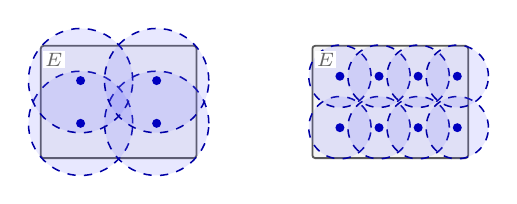
\begin{tikzpicture}[
  scale=0.92,
  every node/.style={font=\scriptsize},
  set/.style={fill=gray!8, draw=black!65, line width=0.65pt},
  ball/.style={fill=blue!55, fill opacity=0.16, draw=blue!65!black, dashed, line width=0.55pt},
  center/.style={circle, fill=blue!75!black, inner sep=1.15pt}
]
  \begin{scope}[shift={(-2.7,0)}]
    \draw[set, rounded corners=1pt] (0,0) rectangle (2.15,1.55);

    \foreach \x/\y in {0.55/0.48,1.60/0.48,0.55/1.07,1.60/1.07} {
      \draw[ball] (\x,\y) circle (0.72);
    }
    \foreach \x/\y in {0.55/0.48,1.60/0.48,0.55/1.07,1.60/1.07} {
      \node[center] at (\x,\y) {};
    }
    \node[black!60, fill=white, inner sep=0.8pt] at (0.18,1.36) {$E$};
  \end{scope}

  \begin{scope}[shift={(1.05,0)}]
    \draw[set, rounded corners=1pt] (0,0) rectangle (2.15,1.55);

    \foreach \x in {0.38,0.92,1.46,2.00} {
      \foreach \y in {0.42,1.13} {
        \draw[ball] (\x,\y) circle (0.43);
      }
    }
    \foreach \x in {0.38,0.92,1.46,2.00} {
      \foreach \y in {0.42,1.13} {
        \node[center] at (\x,\y) {};
      }
    }
    \node[black!60, fill=white, inner sep=0.8pt] at (0.18,1.36) {$E$};
  \end{scope}
\end{tikzpicture}

  \caption{Finite $\varepsilon$- and $\delta$-nets cover $E$, with $0<\delta<\varepsilon$.}
  \label{fig:total-boundedness-finite-cover}
\end{figure}

\begin{definition} \label{def:totally-bounded-metric-space} \hlt{Total Boundedness}\\
Let $(X,d)$ be a metric space. It is \hlt{totally bounded} if, $\forall \varepsilon>0$, $\exists$ a finite set $F\subseteq X$ such that $X\subseteq\bigcup\limits_{x\in F}B_\varepsilon(x)$.\\
$F$ is a finite $\varepsilon$-net. $E\subseteq X$ totally bounded if same condition holds with finite $F\subseteq E$ and $X$.
\end{definition}

\begin{theorem} \label{thm:total-bounded-implies-bounded} \hlt{Total Boundedness Implies Boundedness}\\
Let $X$ be a metric space.
If $X$ is totally bounded, then $X$ is bounded.
\begin{proof}
If $X=\emptyset$, this is trivial. Otherwise cover $X$ by finitely many $1$-balls $B_1(x_i)$ and fix $x_1$.\\
Then $d(x,x_1)<1+\max_i d(x_i,x_1)$ for every $x\in X$.\\
\hlt{Structural Commentary}: One finite cover at scale $1$ gives one global bound.\\
\hlt{Key Insight}: Total boundedness is boundedness with finite control at every scale.
\end{proof}
\end{theorem}

\begin{theorem} \label{thm:compact-complete-totally-bounded} \hlt{Compactness as Complete Finite Resolution}\\
Let $X$ be a metric space. Then, $X$ is compact $\Longleftrightarrow$ $X$ is complete and totally bounded.
\begin{proof}
\begin{enumerate}[label=\roman*.]
\setlength{\itemsep}{0pt}
\item[$(\Rightarrow)$] Let $(p_k)$ be Cauchy in $X$. By Theorem \ref{thm:cauchy-convergence-criterion}, compactness forces $(p_k)$ to converge, so $X$ is complete.\\
Given $\varepsilon>0$, cover $\{B_\varepsilon(x):x\in X\}$ has finite subcover $B_\varepsilon(y_1),\ldots,B_\varepsilon(y_m)$; hence $X$ is totally bounded.
\item[$(\Leftarrow)$] Let $(x_n)\subseteq X$. Choose nested subsequences $(x_k^{(j)})_{k\geq1}$ and points $a_j\in X$ with $x_k^{(j)}\in B_{1/j}(a_j) \ \forall k$.\\
Diagonal $y_j\defeq x_j^{(j)}$ satisfies $y_k,y_\ell\in B_{1/j}(a_j)$ for $k,\ell\geq j$, so it is Cauchy and converges by completeness; hence $X$ is sequentially compact. Now let $\{U_\alpha\}$ cover $X$. If no $\delta>0$ has every $B_\delta(x)$ contained in some $U_\alpha$, choose $x_n$ with $B_{1/n}(x_n)\nsubseteq U_\alpha \ \forall\alpha$. Passing to $x_{n_k}\to x\in U_{\alpha_0}$, and openness gives $B_{1/n_k}(x_{n_k})\subseteq U_{\alpha_0}$ for large $k$, a contradiction. Thus such $\delta$ exists.\\
Choose a finite $\delta/2$-net $\{z_i\}_{i=1}^m$ and $\alpha_i$ with $B_\delta(z_i)\subseteq U_{\alpha_i}$; then $\{U_{\alpha_i}\}_{i=1}^m$ covers $X$.
\end{enumerate}
\hlt{Structural Commentary}: Finite nets plus completeness force compactness.\\
\hlt{Key Insight}: Compact metric spaces are exactly complete spaces visible at every finite scale.
\end{proof}
\end{theorem}

\begin{example} \label{ex:open-interval-cover-without-finite-subcover} \hlt{An Open Cover Without a Finite Subcover}\\
For $x\in(0,1)$, set $O_x\defeq(x/2,1)$. These sets cover $(0,1)$, since $y\in O_x$ whenever $0<x<y<1$.\\
No finite subcollection covers $(0,1)$: if $x'=\min\{x_1,\ldots,x_n\}$, then $(0,x'/2]$ is missed by $O_{x_1}\cup\cdots\cup O_{x_n}$.
\end{example}

\begin{figure}[H]
  \centering
  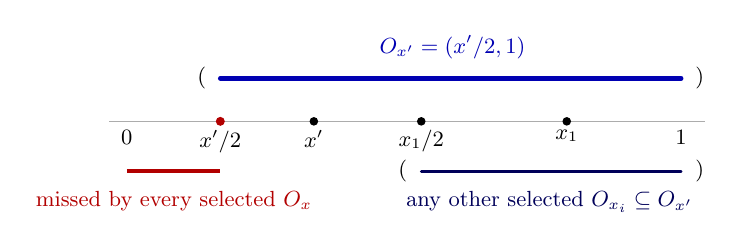
\begin{tikzpicture}[
  scale=0.88,
  transform shape,
  every node/.style={font=\small},
  axis/.style={gray!65, line width=0.55pt},
  cover/.style={blue!70!black, line width=1.7pt, line cap=round},
  subcover/.style={blue!35!black, line width=1.0pt, line cap=round},
  missed/.style={red!70!black, line width=1.35pt},
  point/.style={circle, fill=black, inner sep=1.25pt},
  missedpoint/.style={circle, fill=red!70!black, inner sep=1.3pt}
]
  \draw[axis] (-0.25,0) -- (8.35,0);
  \node[below] at (0,0) {$0$};
  \node[below] at (8,0) {$1$};

  \coordinate (xprimehalf) at (1.35,0);
  \coordinate (xprime) at (2.7,0);
  \coordinate (xonehalf) at (4.25,0);
  \coordinate (xone) at (6.35,0);

  \draw[missed] (0,-0.72) -- (1.35,-0.72);
  \node[red!70!black, below] at (0.68,-0.89) {missed by every selected $O_x$};

  \node[missedpoint] at (xprimehalf) {};
  \node[point] at (xprime) {};
  \node[point] at (xonehalf) {};
  \node[point] at (xone) {};

  \node[below] at (1.35,0) {$x'/2$};
  \node[below] at (2.7,0) {$x'$};
  \node[below] at (4.25,0) {$x_1/2$};
  \node[below] at (6.35,0) {$x_1$};

  \draw[cover] (1.35,0.62) -- (8,0.62);
  \node[anchor=east] at (1.27,0.62) {$($};
  \node[anchor=west] at (8.08,0.62) {$)$};
  \node[blue!70!black, above] at (4.7,0.78) {$O_{x'}=(x'/2,1)$};

  \draw[subcover] (4.25,-0.72) -- (8,-0.72);
  \node[anchor=east] at (4.17,-0.72) {$($};
  \node[anchor=west] at (8.08,-0.72) {$)$};
  \node[blue!35!black, below] at (6.1,-0.89) {any other selected $O_{x_i}\subseteq O_{x'}$};
\end{tikzpicture}

  \caption{For finite choice, $x'=\min_i x_i$ makes $O_{x'}$ largest selected interval, but $(0,x'/2]$ remains uncovered.}
  \label{fig:open-cover-no-finite-subcover}
\end{figure}

\begin{theorem} \label{thm:compactness-independent-of-ambient-space} \hlt{Compactness Is Independent of the Ambient Space}\\
Suppose $K\subseteq Y\subseteq X$, where $X$ is a metric space.\\
Then $K$ is compact relative to $X$ if and only if $K$ is compact relative to $Y$.
\begin{proof}
\begin{enumerate}[label=\roman*.]
\setlength{\itemsep}{0pt}
\item[$(\Rightarrow)$] Let $\{V_\alpha\}_{\alpha\in A}$ be a relative-open cover of $K$ in $Y$.\\
By Theorem \ref{thm:relative-open-intersection-with-open-set}, write $V_\alpha=Y\cap G_\alpha$ with $G_\alpha$ open in $X$. Since $\{G_\alpha\}_{\alpha\in A}$ covers $K$, compactness in $X$ gives a finite $F\subseteq A$ such that $K\subseteq\bigcup_{\alpha\in F}G_\alpha$. As $K\subseteq Y$, $K\subseteq\bigcup_{\alpha\in F}V_\alpha$.
\item[$(\Leftarrow)$] Let $\{G_\alpha\}_{\alpha\in A}$ be an open cover of $K$ in $X$. Then $\{Y\cap G_\alpha\}_{\alpha\in A}$ is a relative-open cover of $K$ in $Y$.\\
Compactness in $Y$ gives a finite $F\subseteq A$ such that $K\subseteq\bigcup_{\alpha\in F}(Y\cap G_\alpha)\subseteq\bigcup_{\alpha\in F}G_\alpha$.
\end{enumerate}
\hlt{Structural Commentary}: Relative covers are ambient covers intersected with $Y$.\\
\hlt{Key Insight}: Openness depends on the ambient space, but compactness does not.
\end{proof}
\end{theorem}

\begin{theorem} \label{thm:compact-subsets-of-metric-spaces-closed} \hlt{Compact Sets Are Closed}\\
Every compact subset of a metric space is closed.
\begin{proof}
Let $K$ be compact in $X$. To prove $K^c$ is open.\\
Fix $p\in K^c$. For each $q\in K$, put $V_q\defeq B_{\frac12d(p,q)}(p)$, $W_q\defeq B_{\frac12d(p,q)}(q)$.\\
The sets $W_q$ form an open cover of $K$, so compactness gives $q_1,\ldots,q_n\in K$ with $K\subseteq W_{q_1}\cup\cdots\cup W_{q_n}$.\\
Let $V\defeq V_{q_1}\cap\cdots\cap V_{q_n}$, which is open by Theorem \ref{thm:metric-open-closed-set-calculus}.\\
No point of $V$ lies in any $W_{q_i}$, by the triangle inequality. Hence $V\cap K=\emptyset$, so $p$ is an interior point of $K^c$.\\
\hlt{Structural Commentary}: Compactness makes the separation finite.\\
\hlt{Key Insight}: A finite subcover lets local point-separations become one open neighborhood of the complement.
\end{proof}
\end{theorem}

\begin{theorem} \label{thm:closed-subsets-of-compact-sets-compact} \hlt{Closed Subsets of Compact Sets Are Compact}\\
Suppose $F\subseteq K\subseteq X$, where $F$ is closed in $X$ and $K$ is compact. Then $F$ is compact.
\begin{proof}
Let $\{V_\alpha\}_{\alpha\in A}$ cover $F$. Since $F^c$ is open, $\{V_\alpha\}_{\alpha\in A}\cup\{F^c\}$ covers $K$.\\
Thus $K\subseteq F^c\cup\bigcup\limits_{\alpha\in F_0}V_\alpha$ for some finite $F_0\subseteq A$, so $F\subseteq\bigcup\limits_{\alpha\in F_0}V_\alpha$.\\
\hlt{Structural Commentary}: The open complement of a closed set covers exactly the part of $K$ not under discussion.\\
\hlt{Key Insight}: Cover $K$, then discard the complement piece.
\end{proof}
\end{theorem}

\begin{corollary} \label{cor:closed-intersection-compact} \hlt{Closed Intersections with Compact Sets}\\
If $F$ is closed in $X$ and $K$ is compact in $X$, then $F\cap K$ is compact.
\begin{proof}
By Theorem \ref{thm:compact-subsets-of-metric-spaces-closed}, $K$ is closed in $X$. Since $F$ is closed, Theorem \ref{thm:metric-open-closed-set-calculus} gives that $F\cap K$ is closed in $X$. Also $F\cap K\subseteq K$, so Theorem \ref{thm:closed-subsets-of-compact-sets-compact} implies $F\cap K$ is compact.\\
\hlt{Structural Commentary}: The intersection is closed inside a compact set.\\
\hlt{Key Insight}: Closed subsets of compact sets remain compact.
\end{proof}
\end{corollary}

\begin{theorem} \label{thm:compact-finite-intersection-property} \hlt{Finite Intersection Property for Compact Sets}\\
Let $\{K_\alpha\}_{\alpha\in A}$ be compact subsets of a metric space $X$, with $A\neq\emptyset$.\\
If $\bigcap\limits_{\alpha\in F}K_\alpha\neq\emptyset$ for every finite nonempty $F\subseteq A$, then $\bigcap\limits_{\alpha\in A}K_\alpha\neq\emptyset$.
\begin{proof}
Choose $\alpha_0\in A$ and suppose $\bigcap\limits_{\alpha\in A}K_\alpha=\emptyset$. Then $K_{\alpha_0}\subseteq\bigcup\limits_{\alpha\in A}K_\alpha^c$. Since each $K_\alpha^c$ is open by Theorem \ref{thm:compact-subsets-of-metric-spaces-closed}, compactness of $K_{\alpha_0}$ gives a finite $F\subseteq A$ with $K_{\alpha_0}\subseteq\bigcup\limits_{\alpha\in F}K_\alpha^c$. Hence $\bigcap\limits_{\alpha\in F\cup\{\alpha_0\}}K_\alpha=\emptyset$, a contradiction.\\
\hlt{Structural Commentary}: Complements turn failure into a finite cover.\\
\hlt{Key Insight}: For compact sets, failure of intersection is already witnessed finitely.
\end{proof}
\end{theorem}

\begin{corollary} \label{cor:nested-nonempty-compact-intersection} \hlt{Nested Nonempty Compact Sets Intersect}\\
If $K_1\supseteq K_2\supseteq K_3\supseteq\cdots$ is a sequence of nonempty compact sets, then $\bigcap_{n=1}^{\infty}K_n\neq\emptyset$.
\begin{proof}
Let $\emptyset\neq F\subseteq\N$ be finite and put $m\defeq\max F$. Since the sequence is nested, $\bigcap\limits_{n\in F}K_n=K_m\neq\emptyset$.\\
Thus $\{K_n\}_{n\in\N}$ has the finite intersection property, so Theorem \ref{thm:compact-finite-intersection-property} gives $\bigcap\limits_{n=1}^{\infty}K_n\neq\emptyset$.\\
\hlt{Structural Commentary}: Nestedness reduces finite intersections to one term.\\
\hlt{Key Insight}: A nested compact sequence has the finite intersection property.
\end{proof}
\end{corollary}

\begin{theorem} \label{thm:infinite-subset-of-compact-has-limit-point} \hlt{Infinite Subsets of Compact Sets Have Limit Points}\\
Let $K\subseteq X$ be compact in a metric space $X$. If $E\subseteq K$ is infinite, then $E^{\operatorname{acc}}\cap K\neq\emptyset$.
\begin{proof}
Suppose $E^{\operatorname{acc}}\cap K=\emptyset$. For each $q\in K$, choose $r_q>0$ such that $B_{r_q}(q)\cap(E\setminus\{q\})=\emptyset$, so $\#(B_{r_q}(q)\cap E)\leq1$.\\
Since $\{B_{r_q}(q):q\in K\}$ covers $K$, compactness gives $q_1,\ldots,q_n\in K$ with $K\subseteq\bigcup\limits_{i=1}^{n}B_{r_{q_i}}(q_i)$.\\
As $E\subseteq K$, $E\subseteq\bigcup\limits_{i=1}^{n}B_{r_{q_i}}(q_i)$, finite union of sets meeting $E$ in at most one point. Thus $E$ is finite, contradiction.\\
\hlt{Structural Commentary}: Compactness makes the local ``at most one point'' obstruction finite.\\
\hlt{Key Insight}: Infinite subsets of compact sets must accumulate somewhere inside the compact set.
\end{proof}
\end{theorem}

\begin{theorem} \label{thm:nested-closed-intervals-intersect} \hlt{Nested Closed Intervals Intersect}\\
If $I_1\supseteq I_2\supseteq I_3\supseteq\cdots$ is a sequence of closed intervals in $\R$, then $\bigcap_{n=1}^{\infty}I_n\neq\emptyset$.
\begin{proof}
Let $I_n=[a_n,b_n]$. The set $\{a_n:n\in\N\}$ is nonempty and bounded above by each $b_m$.\\
Let $x=\sup\{a_n:n\in\N\}$. Then $a_m\leq x\leq b_m$ for every $m$, so $x\in I_m$ for all $m$.\\
\hlt{Structural Commentary}: Completeness traps a common point.\\
\hlt{Key Insight}: The least upper bound of the left endpoints lies in every interval.
\end{proof}
\end{theorem}

\begin{figure}[H]
  \centering
  \begin{tikzpicture}[
  scale=0.88,
  every node/.style={font=\small},
  axis/.style={gray!70, line width=0.55pt},
  interval/.style={blue!70!black, line width=0.85pt},
  tick/.style={gray!70, line width=0.55pt},
  supmark/.style={circle, fill=orange!80!black, inner sep=1.55pt}
]
  \draw[axis] (-4.5,0) -- (4.5,0);

  \coordinate (aone) at (-3.8,0);
  \coordinate (atwo) at (-2.8,0);
  \coordinate (athree) at (-1.8,0);
  \coordinate (an) at (-0.8,0);
  \coordinate (xstar) at (0.2,0);
  \coordinate (bn) at (1.2,0);
  \coordinate (bthree) at (2.2,0);
  \coordinate (btwo) at (3.2,0);
  \coordinate (bone) at (4.2,0);

  \draw[interval] ($(aone)+(0,0.45)$) -- ($(bone)+(0,0.45)$);
  \draw[interval] ($(atwo)+(0,0.85)$) -- ($(btwo)+(0,0.85)$);
  \draw[interval] ($(athree)+(0,1.25)$) -- ($(bthree)+(0,1.25)$);
  \draw[interval] ($(an)+(0,1.65)$) -- ($(bn)+(0,1.65)$);

  \foreach \pt/\lab in {aone/a_1,atwo/a_2,athree/a_3,an/a_n,bn/b_n,bthree/b_3,btwo/b_2,bone/b_1} {
    \draw[tick] (\pt) ++(0,-0.12) -- ++(0,0.24);
    \node[below] at ($(\pt)+(0,-0.12)$) {$\lab$};
  }

  \node[supmark] at (xstar) {};
  \draw[orange!80!black, line width=0.55pt] (xstar) ++(0,-0.22) -- ++(0,2.17);
  \node[above] at ($(xstar)+(0,1.95)$) {$x=\sup\{a_n:n\in\N\}$};

  \node[left] at ($(aone)+(0,0.45)$) {$I_1$};
  \node[left] at ($(atwo)+(0,0.85)$) {$I_2$};
  \node[left] at ($(athree)+(0,1.25)$) {$I_3$};
  \node[left] at ($(an)+(0,1.65)$) {$I_n$};
\end{tikzpicture}

  \caption{For nested closed intervals $[a_n,b_n]$, the supremum of the left endpoints lies between every $a_n$ and $b_n$.}
  \label{fig:nested-closed-intervals-lub}
\end{figure}

\begin{theorem} \label{thm:nested-k-cells-intersect} \hlt{Nested $k$-Cells Intersect}\\
If $I_1\supseteq I_2\supseteq I_3\supseteq\cdots$ is a sequence of $k$-cells in $\R^k$, then $\bigcap_{n=1}^{\infty}I_n\neq\emptyset$.
\begin{proof}
Let $I_n=\{\mathbf{x}\in\R^k:a_{n,j}\leq x_j\leq b_{n,j},\ 1\leq j\leq k\}$. For each coordinate $j$, the intervals $[a_{n,j},b_{n,j}]$ are nested, so Theorem \ref{thm:nested-closed-intervals-intersect} gives a point $x_j^*$ lying in all of them. Then $\mathbf{x}^*=(x_1^*,\ldots,x_k^*)$ lies in every $I_n$.\\
\hlt{Structural Commentary}: A nested cell problem reduces coordinatewise to nested intervals.\\
\hlt{Key Insight}: Choose one persistent coordinate at a time.
\end{proof}
\end{theorem}

\begin{figure}[H]
  \centering
  \begin{tikzpicture}[
  every node/.style={font=\small},
  axis/.style={->, gray!70, line width=0.5pt},
  cell/.style={draw=blue!65!black, fill=blue!12, line width=0.75pt},
  edge/.style={blue!65!black, line width=0.75pt},
  hidden/.style={blue!65!black, dashed, dash pattern=on 2pt off 2pt, line width=0.55pt},
  tick/.style={gray!70, line width=0.5pt}
]
  \begin{scope}
    \draw[axis] (-0.2,0) -- (2.6,0);
    \draw[cell] (0.55,-0.08) rectangle (2.0,0.08);
    \draw[tick] (0.55,-0.18) -- (0.55,0.18);
    \draw[tick] (2.0,-0.18) -- (2.0,0.18);
    \node[below] at (0.55,-0.18) {$a_1$};
    \node[below] at (2.0,-0.18) {$b_1$};
    \node[above] at (1.25,0.35) {$1$-cell};
  \end{scope}

  \begin{scope}[xshift=3.3cm]
    \draw[axis] (-0.2,0) -- (2.8,0);
    \draw[axis] (0,-0.2) -- (0,2.2);
    \draw[cell] (0.7,0.55) rectangle (2.25,1.75);
    \draw[tick] (0.7,-0.12) -- (0.7,0.12);
    \draw[tick] (2.25,-0.12) -- (2.25,0.12);
    \draw[tick] (-0.12,0.55) -- (0.12,0.55);
    \draw[tick] (-0.12,1.75) -- (0.12,1.75);
    \node[below] at (0.7,-0.12) {$a_1$};
    \node[below] at (2.25,-0.12) {$b_1$};
    \node[left] at (-0.12,0.55) {$a_2$};
    \node[left] at (-0.12,1.75) {$b_2$};
    \node[above] at (1.4,2.15) {$2$-cell};
  \end{scope}

  \begin{scope}[xshift=7.0cm]
    \draw[axis] (-0.2,0) -- (2.9,0);
    \draw[axis] (0,-0.2) -- (0,2.25);
    \draw[axis] (-0.1,-0.1) -- (1.1,1.1);
    \coordinate (A) at (0.7,0.55);
    \coordinate (B) at (1.95,0.55);
    \coordinate (C) at (1.95,1.5);
    \coordinate (D) at (0.7,1.5);
    \coordinate (s) at (0.55,0.45);
    \fill[blue!12] (A) -- (B) -- (C) -- (D) -- cycle;
    \fill[blue!8] ($(A)+(s)$) -- ($(B)+(s)$) -- ($(C)+(s)$) -- ($(D)+(s)$) -- cycle;
    \draw[edge] (A) -- (B) -- (C) -- (D) -- cycle;
    \draw[edge] ($(A)+(s)$) -- ($(B)+(s)$) -- ($(C)+(s)$) -- ($(D)+(s)$) -- cycle;
    \draw[edge] (B) -- ($(B)+(s)$);
    \draw[edge] (C) -- ($(C)+(s)$);
    \draw[edge] (D) -- ($(D)+(s)$);
    \draw[hidden] (A) -- ($(A)+(s)$);
    \node[below] at (0.7,-0.08) {$a_1$};
    \node[below] at (2.5,-0.08) {$b_1$};
    \node[left] at (-0.08,0.55) {$a_2$};
    \node[left] at (-0.08,1.5) {$b_2$};
    \node[right] at ($(B)+(s)+(0.05,0)$) {$b_3$};
    \node[above] at (1.45,2.15) {$3$-cell};
  \end{scope}
\end{tikzpicture}

  \caption{A $1$-cell is a closed interval, a $2$-cell is a coordinate rectangle, and a $3$-cell is a coordinate box.}
  \label{fig:k-cell-low-dimensional-examples}
\end{figure}

\begin{theorem} \label{thm:k-cells-compact} \hlt{$k$-Cells Are Compact}\\
Every $k$-cell in $\R^k$ is compact.
\begin{proof}
Let $I=\{\mathbf{x}:a_j\leq x_j\leq b_j,\ 1\leq j\leq k\}$ and set $\delta\defeq\left(\sum
\limits_{j=1}^{k}(b_j-a_j)^2\right)^{1/2}$. Suppose an open cover $\{G_\alpha\}$ of $I$ has no finite subcover. Bisect each coordinate interval. Among the resulting $2^k$ subcells, at least one cannot be finitely covered by the $G_\alpha$; call it $I_1$. Continue inductively, obtaining nested cells $I\supseteq I_1\supseteq I_2\supseteq\cdots$ such that no $I_n$ is finitely covered and every two points of $I_n$ are within $2^{-n}\delta$ of each other.\\
By Theorem \ref{thm:nested-k-cells-intersect}, choose $\mathbf{x}^*\in\bigcap_n I_n$. Since $\{G_\alpha\}$ covers $I$, some $G_\alpha$ contains $\mathbf{x}^*$. Because $G_\alpha$ is open, $B_r(\mathbf{x}^*)\subseteq G_\alpha$ for some $r>0$. By the Archimedean property in Theorem \ref{thm:archimedean-and-rational-density}, choose $n$ with $n>\delta/r$; since $2^n\geq n$, we have $2^{-n}\delta<r$. Then $I_n\subseteq G_\alpha$, contradicting the construction of $I_n$.\\
\hlt{Structural Commentary}: Repeated bisection traps a point in cells whose diameters shrink to zero.\\
\hlt{Key Insight}: An open set around the trapped point eventually contains the whole small cell.
\end{proof}
\end{theorem}

\begin{figure}[H]
  \centering
  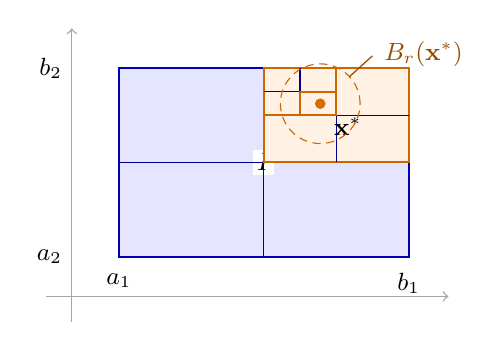
\begin{tikzpicture}[
  scale=0.92,
  every node/.style={font=\small},
  axis/.style={->, gray!70, line width=0.5pt},
  cell/.style={draw=blue!70!black, fill=blue!10, line width=0.75pt},
  subcell/.style={draw=blue!55!black, line width=0.45pt},
  focus/.style={draw=orange!80!black, fill=orange!10, line width=0.75pt},
  point/.style={circle, fill=orange!85!black, inner sep=1.35pt}
]
  \draw[axis] (-0.35,0) -- (5.2,0);
  \draw[axis] (0,-0.35) -- (0,3.7);

  \coordinate (A) at (0.65,0.55);
  \coordinate (B) at (4.65,0.55);
  \coordinate (C) at (4.65,3.15);
  \coordinate (D) at (0.65,3.15);

  \draw[cell] (A) rectangle (C);
  \node[fill=white, inner sep=1.5pt] at (2.65,1.85) {$I$};

  \draw[subcell] (2.65,0.55) -- (2.65,3.15);
  \draw[subcell] (0.65,1.85) -- (4.65,1.85);

  \draw[focus] (2.65,1.85) rectangle (4.65,3.15);
  \draw[subcell] (3.65,1.85) -- (3.65,3.15);
  \draw[subcell] (2.65,2.5) -- (4.65,2.5);

  \draw[focus] (2.65,2.5) rectangle (3.65,3.15);
  \draw[subcell] (3.15,2.5) -- (3.15,3.15);
  \draw[subcell] (2.65,2.825) -- (3.65,2.825);

  \draw[focus] (3.15,2.5) rectangle (3.65,2.825);
  \node[point,label=below right:$\mathbf{x}^\ast$] at (3.43,2.66) {};

  \node[below] at (0.65,0.45) {$a_1$};
  \node[below] at (4.65,0.45) {$b_1$};
  \node[left] at (0.0,0.55) {$a_2$};
  \node[left] at (0.0,3.15) {$b_2$};

  \draw[orange!80!black, dashed, dash pattern=on 3pt off 2pt] (3.43,2.66) circle (0.55);
  \draw[orange!60!black, line width=0.45pt] (3.83,3.03) -- (4.15,3.32);
  \node[orange!60!black, anchor=west] at (4.18,3.34) {$B_r(\mathbf{x}^\ast)$};
\end{tikzpicture}

  \caption{Repeated bisection traps a point.}
  \label{fig:k-cell-bisection-compactness}
\end{figure}

\begin{lemma} \label{lem:bounded-rk-set-contained-in-k-cell} \hlt{Bounded Euclidean Sets Fit in $k$-Cells}\\
Every bounded subset $E\subseteq\R^k$ is contained in some $k$-cell.
\begin{proof}
If $E=\emptyset$, any $k$-cell contains $E$. Suppose $E\neq\emptyset$. By Definition \ref{def:bounded-and-perfect-metric-sets}, choose $\mathbf{q}=(q_1,\ldots,q_k)\in\R^k$ and $M>0$ such that $\norm{\mathbf{p}-\mathbf{q}}_2<M$ for all $\mathbf{p}\in E$. Let $I\defeq\{\mathbf{x}=(x_1,\ldots,x_k):q_j-M\leq x_j\leq q_j+M,\ 1\leq j\leq k\}$.\\
For $\mathbf{p}=(p_1,\ldots,p_k)\in E$, $\abs{p_j-q_j}\leq\norm{\mathbf{p}-\mathbf{q}}_2<M$ for each $j$, so $\mathbf{p}\in I$.\\
Thus $E\subseteq I$, and $I$ is a $k$-cell by Definition \ref{def:euclidean-intervals-cells-balls-convex}.\\
\hlt{Structural Commentary}: A Euclidean ball centered at $\mathbf{q}$ sits inside the coordinate box with side half-length $M$.\\
\hlt{Key Insight}: Boundedness supplies one radius; coordinates turn it into interval bounds.
\end{proof}
\end{lemma}

\begin{theorem} \label{thm:heine-borel-rk} \hlt{Heine--Borel in $\R^k$}\\
For $E\subseteq\R^k$, any one of the following three properties implies the other two:
\begin{enumerate}[label=(\roman*)]
\setlength{\itemsep}{0pt}
\item $E$ is closed and bounded;
\item $E$ is compact;
\item every infinite subset of $E$ has a limit point in $E$.
\end{enumerate}
\begin{proof}
\begin{enumerate}[label=(\roman*)]
\setlength{\itemsep}{0pt}
\item[$(i)$]$\Rightarrow(ii)$: Since $E$ is bounded, Lemma \ref{lem:bounded-rk-set-contained-in-k-cell} gives $E\subseteq I$ for some $k$-cell $I$. By Theorem \ref{thm:k-cells-compact}, $I$ is compact; since $E$ is closed, Theorem \ref{thm:closed-subsets-of-compact-sets-compact} gives that $E$ is compact.
\item[$(ii)$]$\Rightarrow(iii)$: This is Theorem \ref{thm:infinite-subset-of-compact-has-limit-point}.
\item[$(iii)$]$\Rightarrow(i)$: If $E$ is unbounded, choose $\mathbf{x}_n\in E$ with $\norm{\mathbf{x}_n}_2>n$ and set $S\defeq\{\mathbf{x}_n:n\in\N\}$. If $\mathbf{x}_n\in B_R(\mathbf{y})$, then $n<\norm{\mathbf{y}}_2+R$; hence $S$ has no limit point, contradicting (iii). Thus $E$ is bounded. If $E$ is not closed, choose $\mathbf{x}_0\in E^{\operatorname{acc}}\setminus E$ and $\mathbf{x}_n\in E$ with $0<\norm{\mathbf{x}_n-\mathbf{x}_0}_2<1/n$. Then $S\defeq\{\mathbf{x}_n:n\in\N\}$ is infinite and $S^{\operatorname{acc}}\subseteq\{\mathbf{x}_0\}\subseteq E^c$, contradicting (iii). Thus $E$ is closed.
\end{enumerate}
\hlt{Structural Commentary}: In $\R^k$, the three tests coincide.\\
\hlt{Key Insight}: Heine--Borel is the bridge between open-cover compactness and Euclidean bounded geometry.
\end{proof}
\end{theorem}

\begin{corollary} \label{cor:heine-borel-real-line-sequential-form} \hlt{Heine--Borel on the Real Line}\\
For $E\subseteq\R$, the following are equivalent:
\begin{enumerate}[label=(\roman*)]
\setlength{\itemsep}{0pt}
\item $E$ is closed and bounded;
\item $E$ is compact;
\item every sequence in $E$ has a subsequence converging to a point of $E$.
\end{enumerate}
\begin{proof}
\begin{enumerate}[label=(\roman*).]
\setlength{\itemsep}{0pt}
\item[$(i)$]$\Rightarrow (ii)$ Since $E\subseteq\R=\R^1$ is closed and bounded, Theorem \ref{thm:heine-borel-rk} with $k=1$ implies $E$ is compact.
\item[$(ii)$]$\Rightarrow (iii)$ Compactness and Theorem \ref{thm:compact-complete-totally-bounded} give convergent subsequence; compactness keeps limit in $E$.
\item[$(iii)$]$\Rightarrow (i)$ Let $F\subseteq E$ be infinite. Choose distinct $x_n\in F$ using Principle \ref{princ:axiom-of-choice-analysis}. By (iii), some $x_{n_j}\to x\in E$. Since the $x_n$ are distinct, $x$ is a limit point of $F$ in the sense of Definition \ref{def:metric-topology-core-definitions}. Hence every infinite subset of $E$ has a limit point in $E$, so Theorem \ref{thm:heine-borel-rk} gives that $E$ is closed and bounded.
\end{enumerate}
\hlt{Structural Commentary}: Real-line compactness equals closed-bounded sequential compactness.\\
\hlt{Key Insight}: Closed bounded sets keep sequences from escaping.
\end{proof}
\end{corollary}

\begin{theorem} \label{thm:weierstrass-limit-point-rk} \hlt{Weierstrass Limit-Point Theorem}\\
Every bounded infinite subset of $\R^k$ has a limit point in $\R^k$.
\begin{proof}
By Lemma \ref{lem:bounded-rk-set-contained-in-k-cell}, a bounded set $E$ lies in some $k$-cell $I$. By Theorem \ref{thm:k-cells-compact}, $I$ is compact.\\
Since $E$ is an infinite subset of $I$, Theorem \ref{thm:infinite-subset-of-compact-has-limit-point} gives a limit point of $E$ in $I\subseteq\R^k$.\\
\hlt{Structural Commentary}: Boundedness places the set inside a compact cell.\\
\hlt{Key Insight}: Compact cells force bounded infinite sets to accumulate.
\end{proof}
\end{theorem}

\begin{theorem} \label{thm:nonempty-perfect-subset-rk-uncountable} \hlt{Perfect Sets Are Uncountable}\\
Every nonempty perfect subset of $\R^k$ is uncountable.
\begin{proof}
Assume $P=\{\mathbf{x}_1,\mathbf{x}_2,\ldots\}$. Choose a neighborhood $V_1$ with $V_1\cap P\neq\emptyset$.\\
Inductively, since $P\cap V_n$ contains infinitely many points by Theorem \ref{thm:limit-point-neighborhoods-infinitely-many}, choose $\mathbf{y}_n\in P\cap V_n$ with $\mathbf{y}_n\neq\mathbf{x}_n$ and then a neighborhood $V_{n+1}$ of $\mathbf{y}_n$ such that $\overline{V}_{n+1}\subseteq V_n$ and $\mathbf{x}_n\notin\overline{V}_{n+1}$.\\
Put $K_n\defeq\overline{V}_n\cap P$. Then $K_n$ is nonempty, compact, and $K_{n+1}\subseteq K_n$. By Corollary \ref{cor:nested-nonempty-compact-intersection}, choose $\mathbf{z}\in\bigcap\limits_{n=1}^{\infty}K_n$. For each $n$, $\mathbf{z}\in K_{n+1}$ but $\mathbf{x}_n\notin K_{n+1}$, so $\mathbf{z}\neq\mathbf{x}_n$ for all $n$, contradicting the enumeration.\\
\hlt{Structural Commentary}: Nested compact sets dodge the list.\\
\hlt{Key Insight}: Perfectness gives new points; compactness keeps one.
\end{proof}
\end{theorem}

\begin{figure}[H]
  \centering
  \begin{tikzpicture}[
  every node/.style={font=\small},
  axis/.style={gray!65, line width=0.55pt},
  interval/.style={blue!70!black, line width=1.35pt},
  smallinterval/.style={orange!80!black, line width=1.45pt},
  guide/.style={gray!55, dashed, line width=0.45pt},
  point/.style={circle, fill=black, inner sep=1.45pt}
]
  \draw[axis] (-0.25,0) -- (7.25,0);

  \coordinate (iOneL) at (0.45,0);
  \coordinate (iOneR) at (6.85,0);
  \coordinate (xone) at (2.45,0);
  \coordinate (iTwoL) at (4.35,0);
  \coordinate (ytwo) at (5.05,0);
  \coordinate (iTwoR) at (5.85,0);

  \draw[interval] ($(iOneL)+(0,0.62)$) -- ($(iOneR)+(0,0.62)$);
  \draw[interval] ($(iOneL)+(0,0.34)$) -- ($(iOneL)+(0,0.90)$);
  \draw[interval] ($(iOneR)+(0,0.34)$) -- ($(iOneR)+(0,0.90)$);
  \node[blue!70!black, above] at (3.65,0.92) {$I_1$};

  \draw[smallinterval] ($(iTwoL)+(0,-0.50)$) -- ($(iTwoR)+(0,-0.50)$);
  \draw[smallinterval] ($(iTwoL)+(0,-0.76)$) -- ($(iTwoL)+(0,-0.24)$);
  \draw[smallinterval] ($(iTwoR)+(0,-0.76)$) -- ($(iTwoR)+(0,-0.24)$);
  \node[orange!80!black, below] at ($(ytwo)+(0,-0.78)$) {$I_2$};

  \draw[guide] (iTwoL) -- ($(iTwoL)+(0,-0.50)$);
  \draw[guide] (iTwoR) -- ($(iTwoR)+(0,-0.50)$);

  \node[point] at (xone) {};
  \node[below] at (xone) {$x_1$};

  \node[point] at (ytwo) {};
  \node[above] at (ytwo) {$y_2\in P$};

  \node[gray!65] at (3.40,-0.50) {$x_1\notin I_2$};
\end{tikzpicture}

  \caption{Choose $y_2\in P\cap I_1$ with $y_2\neq x_1$, then take a smaller interval $I_2\subseteq I_1$ around $y_2$ that avoids $x_1$.}
  \label{fig:perfect-set-nested-interval-avoidance}
\end{figure}

\begin{corollary} \label{cor:closed-intervals-and-reals-uncountable} \hlt{Intervals and the Real Line Are Uncountable}\\
Every interval $[a,b]\subseteq\R$ with $a<b$ is uncountable. In particular, $\R$ is uncountable.
\begin{proof}
The interval $I\defeq[a,b]$ is a nonempty $1$-cell, hence compact by Theorem \ref{thm:k-cells-compact} and closed by Theorem \ref{thm:compact-subsets-of-metric-spaces-closed}. For every $x\in I$ and $\varepsilon>0$, $I\cap \bigl(B_{\varepsilon}(x)\setminus\{x\}\bigr)\neq\emptyset$, so $I$ is perfect. Theorem \ref{thm:nonempty-perfect-subset-rk-uncountable} gives that $I$ is uncountable. If $\R$ were countable, then $I\subseteq\R$ would be countable, a contradiction.\\
\hlt{Structural Commentary}: Closed intervals are perfect compact sets.\\
\hlt{Key Insight}: One closed interval already forces $\R$ to be uncountable.
\end{proof}
\end{corollary}

\begin{figure}[H]
  \centering
  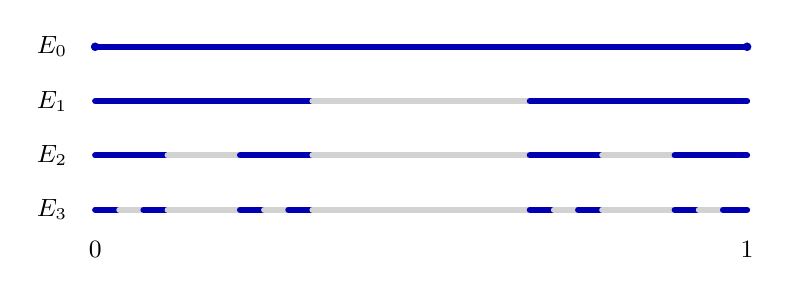
\begin{tikzpicture}[
  every node/.style={font=\small},
  stage/.style={blue!70!black, line width=2.2pt, line cap=round},
  gap/.style={gray!35, line width=2.2pt, line cap=round},
  endpoint/.style={circle, fill=blue!70!black, inner sep=1.1pt},
  scale=0.92
]
  \node[anchor=east] at (-0.25,0) {$E_0$};
  \draw[stage] (0,0) -- (9,0);

  \node[anchor=east] at (-0.25,-0.75) {$E_1$};
  \draw[stage] (0,-0.75) -- (3,-0.75);
  \draw[gap] (3,-0.75) -- (6,-0.75);
  \draw[stage] (6,-0.75) -- (9,-0.75);

  \node[anchor=east] at (-0.25,-1.5) {$E_2$};
  \draw[stage] (0,-1.5) -- (1,-1.5);
  \draw[gap] (1,-1.5) -- (2,-1.5);
  \draw[stage] (2,-1.5) -- (3,-1.5);
  \draw[gap] (3,-1.5) -- (6,-1.5);
  \draw[stage] (6,-1.5) -- (7,-1.5);
  \draw[gap] (7,-1.5) -- (8,-1.5);
  \draw[stage] (8,-1.5) -- (9,-1.5);

  \node[anchor=east] at (-0.25,-2.25) {$E_3$};
  \draw[stage] (0,-2.25) -- (1/3,-2.25);
  \draw[gap] (1/3,-2.25) -- (2/3,-2.25);
  \draw[stage] (2/3,-2.25) -- (1,-2.25);
  \draw[gap] (1,-2.25) -- (2,-2.25);
  \draw[stage] (2,-2.25) -- (7/3,-2.25);
  \draw[gap] (7/3,-2.25) -- (8/3,-2.25);
  \draw[stage] (8/3,-2.25) -- (3,-2.25);
  \draw[gap] (3,-2.25) -- (6,-2.25);
  \draw[stage] (6,-2.25) -- (19/3,-2.25);
  \draw[gap] (19/3,-2.25) -- (20/3,-2.25);
  \draw[stage] (20/3,-2.25) -- (7,-2.25);
  \draw[gap] (7,-2.25) -- (8,-2.25);
  \draw[stage] (8,-2.25) -- (25/3,-2.25);
  \draw[gap] (25/3,-2.25) -- (26/3,-2.25);
  \draw[stage] (26/3,-2.25) -- (9,-2.25);

  \foreach \x in {0,9} {
    \node[endpoint] at (\x,0) {};
  }
  \node[below] at (0,-2.55) {$0$};
  \node[below] at (9,-2.55) {$1$};
\end{tikzpicture}

  \caption{The first stages $E_0,E_1,E_2,E_3$ in the Cantor-set construction.}
  \label{fig:cantor-set-first-stages}
\end{figure}

\begin{example} \label{ex:cantor-set} \hlt{The Cantor Set}\\
Let $E_0=[0,1]$. Remove the open middle third $(1/3,2/3)$ and call the remaining set $E_1$. Continue by removing the open middle third from each interval component, so
\begin{align}
E_1&=[0,1/3]\cup[2/3,1], \nonumber\\
E_2&=[0,1/9]\cup[2/9,3/9]\cup[6/9,7/9]\cup[8/9,1]. \nonumber
\end{align}
Then $E_n$ is a union of $2^n$ compact intervals of length $3^{-n}$ and $E_1\supseteq E_2\supseteq E_3\supseteq\cdots$.\\
The \hlt{Cantor set} is $P\defeq\bigcap\limits_{n=1}^{\infty}E_n$. By Corollary \ref{cor:nested-nonempty-compact-intersection}, $P\neq\emptyset$. Since each $E_n$ is closed and $P\subseteq E_1$, $P$ is a closed subset of the compact set $E_1$, hence compact.\\
If $J\subseteq[0,1]$ is nonempty open interval, for some $m\in\N$ and $k\geq0$, $R_{m,k}\defeq\left(\frac{3k+1}{3^m},\frac{3k+2}{3^m}\right)\subseteq J$ and $R_{m,k}\cap P=\emptyset$.\\
Thus $P$ contains no nontrivial interval. Finally, let $x\in P$ and let $U$ be an interval neighborhood of $x$. If $I_n(x)$ is the component of $E_n$ containing $x$, choose $n$ with $I_n(x)\subseteq U$. An endpoint $y\neq x$ of $I_n(x)$ lies in $P$, so $U\cap(P\setminus\{x\})\neq\emptyset$. Hence $P$ is perfect.\\
\hlt{Structural Commentary}: The Cantor set is built by nested compact deletion, not by listing points.\\
\hlt{Key Insight}: It is compact and perfect, but contains no interval.
\end{example}

\begin{definition} \label{def:fsigma-gdelta-nowhere-dense} \hlt{$F_\sigma$, $G_\delta$, and Nowhere-Dense Sets}\\
For subsets of a metric space $X$:
\begin{enumerate}[label=(\roman*)]
\setlength{\itemsep}{0pt}
\item $A$ is an \hlt{$F_\sigma$ set} if $A=\bigcup_{n=1}^{\infty}F_n$ for closed sets $F_n$.
\item $B$ is a \hlt{$G_\delta$ set} if $B=\bigcap_{n=1}^{\infty}G_n$ for open sets $G_n$.
\item $E$ is \hlt{nowhere dense} if $(\overline{E})^\circ=\emptyset$; equivalently, no nonempty open set is contained in $\overline{E}$.
\end{enumerate}
For $X=\R$, this says exactly that $\overline{E}$ contains no nonempty open interval.
\end{definition}

\begin{definition} \label{def:first-category-set} \hlt{First Category}\\
A set $E\subseteq X$ is \hlt{of first category}, \hlt{meager}, or \hlt{thin}, if covered by countably many nowhere-dense sets: $E\subseteq \bigcup\limits_{n=1}^{\infty}E_n$.\\
The Baire Category Theorem states that a nonempty complete metric space is not first category in itself.
\end{definition}

\begin{definition} \label{def:residual-thick-generic-set} \hlt{Residual, Thick, and Generic Sets}\\
A set $G\subseteq X$ is \hlt{residual}, or \hlt{thick}, if it contains a countable intersection $\bigcap\limits_{n=1}^{\infty}O_n$ of dense open subsets of $X$.\\
A property is \hlt{generic} in $X$ if the set of points satisfying it is residual.\\
By Theorem \ref{thm:dense-open-baire-complete-metric-space}, residual subsets of a complete metric space are dense.\\
In this sense, meager sets are topologically small and residual sets are topologically large.
\end{definition}

\begin{theorem} \label{thm:dense-open-baire-real-line}\label{thm:completeness-and-baire-source-todo} \hlt{Dense Open Intersections in $\R$}\\
If $G_1,G_2,G_3,\ldots$ are dense open subsets of $\R$, then $\bigcap_{n=1}^{\infty}G_n\neq\emptyset$.
\begin{proof}
We construct nested closed intervals. Since $G_1$ is dense and open, $G_1\cap(0,1)$ contains a nonempty open interval; choose a closed interval $I_1\subseteq G_1\cap(0,1)$ with nonempty interior.\\
Given $I_n=[a_n,b_n]$, density of $G_{n+1}$ gives a point of $G_{n+1}$ in $(a_n,b_n)$. Since $G_{n+1}$ is open, choose a closed interval $I_{n+1}\subseteq G_{n+1}\cap(a_n,b_n)$ with nonempty interior and length $<1/(n+1)$.\\
Then $I_1\supseteq I_2\supseteq I_3\supseteq\cdots$, so Theorem \ref{thm:nested-closed-intervals-intersect} gives $x\in\bigcap_n I_n$. Since $I_n\subseteq G_n$ for every $n$, this $x$ lies in $\bigcap_nG_n$.\\
\hlt{Structural Commentary}: Dense openness builds nested intervals; completeness keeps a limit point.\\
\hlt{Key Insight}: A countable dense-open intersection cannot be destroyed one interval at a time.
\end{proof}
\end{theorem}

\begin{theorem} \label{thm:dense-open-baire-complete-metric-space} \hlt{Dense Open Intersections in Complete Metric Spaces}\\
Let $(X,d)$ be complete, let $O_1,O_2,\ldots$ be dense open subsets of $X$, and let $U\subseteq X$ be nonempty and open.\\
Then $U\cap\bigcap\limits_{n=1}^{\infty}O_n\neq\emptyset$. Consequently, $\bigcap\limits_{n=1}^{\infty}O_n$ is dense in $X$.
\begin{proof}
Choose $x_1\in U\cap O_1$ and $0<r_1<1$ with $C_1\defeq\overline{B}_{r_1}(x_1)\subseteq U\cap O_1$.\\
Inductively, if $C_n=\overline{B}_{r_n}(x_n)\subseteq U\cap O_1\cap\cdots\cap O_n$ and $0<r_n<2^{-n}$, density and openness of $O_{n+1}$ give $x_{n+1}\in B_{r_n}(x_n)\cap O_{n+1}$ and $0<r_{n+1}<2^{-(n+1)}$ such that $C_{n+1}\defeq\overline{B}_{r_{n+1}}(x_{n+1})\subseteq B_{r_n}(x_n)\cap O_{n+1}$.\\
Then $C_{n+1}\subseteq C_n$. If $m>n$, then $x_m\in B_{r_n}(x_n)$, so $d(x_m,x_n)<2^{-n}$; hence $(x_n)$ is Cauchy. Let $x_n\to x$.\\
Since each $C_n$ is closed and contains all sufficiently late $x_m$, we have $x\in C_n$ for every $n$. Thus $x\in U\cap\bigcap_nO_n$.\\
Since every nonempty open $U$ meets $\bigcap_nO_n$, the intersection is dense.\\
\hlt{Structural Commentary}: The interval proof becomes a nested closed-ball proof.\\
\hlt{Key Insight}: Dense open sets choose the next ball; completeness supplies the limiting point.
\end{proof}
\end{theorem}

\begin{figure}[H]
  \centering
  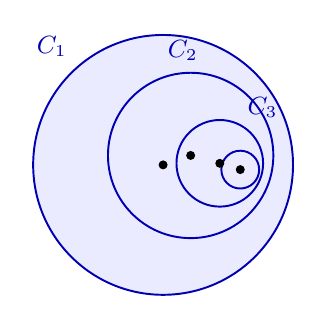
\begin{tikzpicture}[
  every node/.style={font=\small},
  ball/.style={draw=blue!70!black, fill=blue!8, line width=0.7pt},
  center/.style={circle, fill=black, inner sep=1.15pt}
]
  \draw[ball] (0,0) circle (1.65);
  \draw[ball] (0.35,0.12) circle (1.05);
  \draw[ball] (0.72,0.02) circle (0.55);
  \draw[ball] (0.98,-0.06) circle (0.24);

  \node[center] at (0,0) {};
  \node[center] at (0.35,0.12) {};
  \node[center] at (0.72,0.02) {};
  \node[center] at (0.98,-0.06) {};

  \node[blue!70!black, above left] at (-1.1,1.25) {$C_1$};
  \node[blue!70!black, above] at (0.25,1.20) {$C_2$};
  \node[blue!70!black, above right] at (0.95,0.48) {$C_3$};
\end{tikzpicture}

  \caption{Nested closed balls shrink to \(p\).}
  \label{fig:baire-nested-closed-balls}
\end{figure}

\begin{theorem} \label{thm:baire-category-complete-metric-space} \hlt{Baire Category Theorem for Complete Metric Spaces}\\
A nonempty complete metric space is not the union of a countable collection of nowhere-dense sets.
\begin{proof}
Suppose $X=\bigcup_nE_n$ with each $E_n$ nowhere dense, and set $O_n\defeq(\overline{E_n})^c$.\\
Then each $O_n$ is dense open: it is open, and every nonempty open set meets it because no such set lies in $\overline{E_n}$.\\
By Theorem \ref{thm:dense-open-baire-complete-metric-space}, choose $x\in\bigcap_nO_n$. Then $x\notin E_n$ for all $n$, contradicting $X=\bigcup_nE_n$.\\
\hlt{Structural Commentary}: Countably many nowhere-dense sets have dense open complements.\\
\hlt{Key Insight}: Completeness forbids countable assembly from thin pieces.
\end{proof}
\end{theorem}

\begin{perspective} \label{per:baire-category-in-function-spaces} \hlt{Category in Function Spaces}\\
Baire category is a theorem about complete metric spaces, not just $\R$.\\
It will be reused for complete function spaces under the supremum metric.
\end{perspective}

\begin{theorem} \label{thm:baire-category-real-line} \hlt{Baire's Theorem for $\R$}\\
The real line $\R$ cannot be written as a countable union of nowhere-dense sets.
\begin{proof}
Assume $\R=\bigcup_nE_n$ with each $E_n$ nowhere dense, and set $U_n\defeq(\overline{E_n})^c$.\\
Each $U_n$ is dense open: it is open, and every nonempty interval meets it because no such interval lies in $\overline{E_n}$.\\
By Theorem \ref{thm:dense-open-baire-real-line}, choose $x\in\bigcap_nU_n$. Then $x\notin E_n$ for all $n$, contradicting $\R=\bigcup_nE_n$.\\
\hlt{Structural Commentary}: Nowhere-dense sets have dense open complements.\\
\hlt{Key Insight}: Countably many thin sets cannot exhaust the real line.
\end{proof}
\end{theorem}

\begin{corollary} \label{cor:rationals-not-gdelta-irrationals-not-fsigma} \hlt{Rationals and Irrationals by Category}\\
The set $\Q$ is $F_\sigma$ but not $G_\delta$. The set $\R\setminus\Q$ is $G_\delta$ but not $F_\sigma$.
\begin{proof}
Write $\Q=\{q_1,q_2,\ldots\}$. Since singletons are closed, $\Q=\bigcup_n\{q_n\}$ is $F_\sigma$, and $\R\setminus\Q=\bigcap_n(\{q_n\})^c$ is $G_\delta$.\\
If $\Q=\bigcap_nG_n$ with each $G_n$ open, then each $G_n$ is dense because it contains the dense set $\Q$. Set $H_n\defeq G_n\setminus\{q_n\}$.\\
Each $H_n$ is dense open, so Theorem \ref{thm:dense-open-baire-real-line} gives a point of $\bigcap_nH_n$. But $\bigcap_nH_n=\emptyset$, since $\bigcap_nG_n=\Q$ and $q_n$ is removed at stage $n$. Hence $\Q$ is not $G_\delta$. Therefore $\R\setminus\Q$ is not $F_\sigma$, or else its complement $\Q$ would be $G_\delta$.\\
\hlt{Structural Commentary}: Category separates the familiar countable dense set from its dense complement.\\
\hlt{Key Insight}: Dense is not the same as large in the Baire-category sense.
\end{proof}
\end{corollary}

\begin{method} \label{meth:baire-category-proof-patterns} \hlt{Baire-Category Proof Patterns}
\begin{enumerate}[label=(\roman*)]
\setlength{\itemsep}{0pt}
\item \hlt{Dense-open intersection}: build nested closed intervals $I_n\subseteq G_n$ and apply Theorem \ref{thm:nested-closed-intervals-intersect}.
\item \hlt{Complete metric version}: build nested closed balls $C_{n+1}\subseteq C_n$ with $r_n\to0$ and use completeness.
\item \hlt{Nowhere dense}: replace $E$ by the dense open set $(\overline{E})^c$.
\item \hlt{First category}: show the exceptional set is contained in $\bigcup_n E_n$ with each $E_n$ nowhere dense.
\item \hlt{Residual/generic}: show the desired property contains $\bigcap_n O_n$ with each $O_n$ dense open.
\item \hlt{$F_\sigma/G_\delta$ complements}: pass between countable unions and intersections by De Morgan's laws.
\end{enumerate}
\end{method}
